% ============================================================================
%  front/cover.tex — جلدِ جزوه (تماماً تک‌صفحه‌ای و تمام‌نگاشت)
%  همهٔ عناصرِ جلد در لایهٔ overlay قرار گرفته‌اند تا هیچ‌کدام به صفحهٔ دوم
%  سرریز نکنند و سبکِ سرصفحه/پاصفحه نیز روی جلد اعمال نشود.
% ============================================================================
\thispagestyle{JEmpty}%
\begin{tikzpicture}[remember picture, overlay]
  % زمینهٔ نیلیِ تمام‌صفحه
  \fill[JPrimary] (current page.south west) rectangle (current page.north east);

  % نوارِ تزئینیِ بالا
  \begin{scope}
    \clip ([yshift=-4.35cm]current page.north west) rectangle
          ([yshift=0.05cm]current page.north east);
    \node[anchor=north, inner sep=0pt] at ([yshift=0.05cm]current page.north)
      {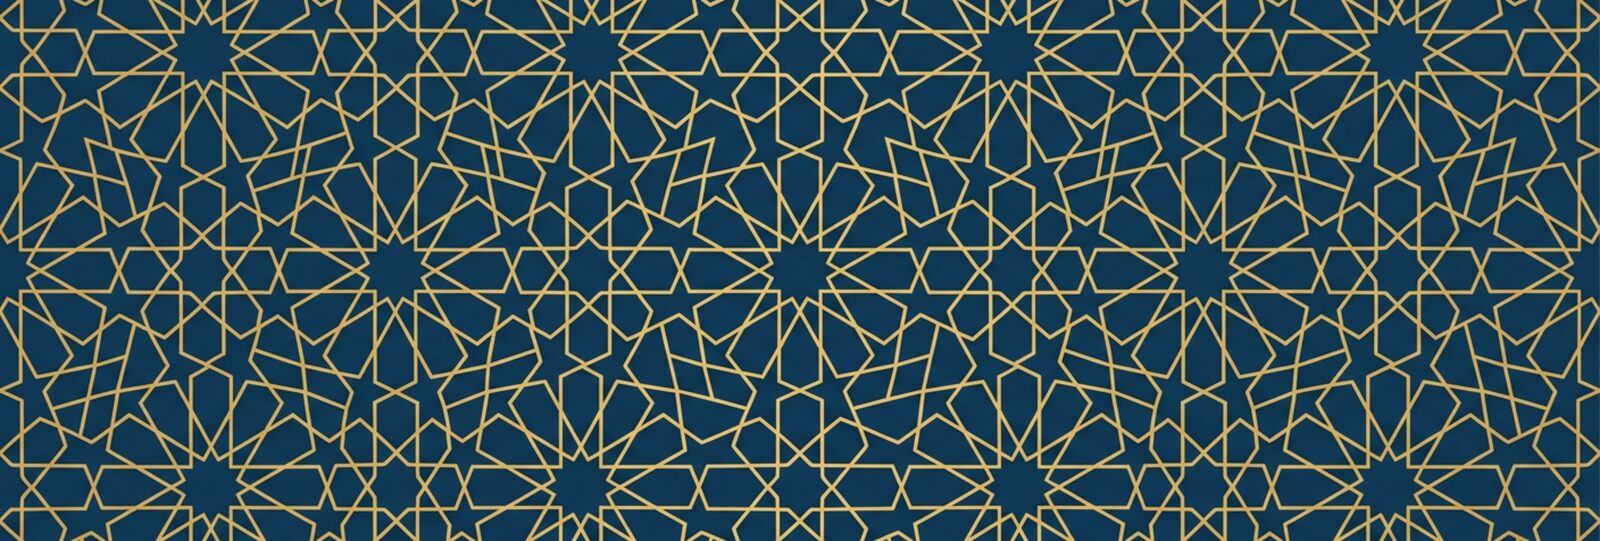
\includegraphics[width=21.4cm]{assets/band-strip.jpg}};
  \end{scope}

  % نوارِ تزئینیِ پایین
  \begin{scope}
    \clip ([yshift=4.35cm]current page.south west) rectangle
          ([yshift=-0.05cm]current page.south east);
    \node[anchor=south, inner sep=0pt] at ([yshift=-0.05cm]current page.south)
      {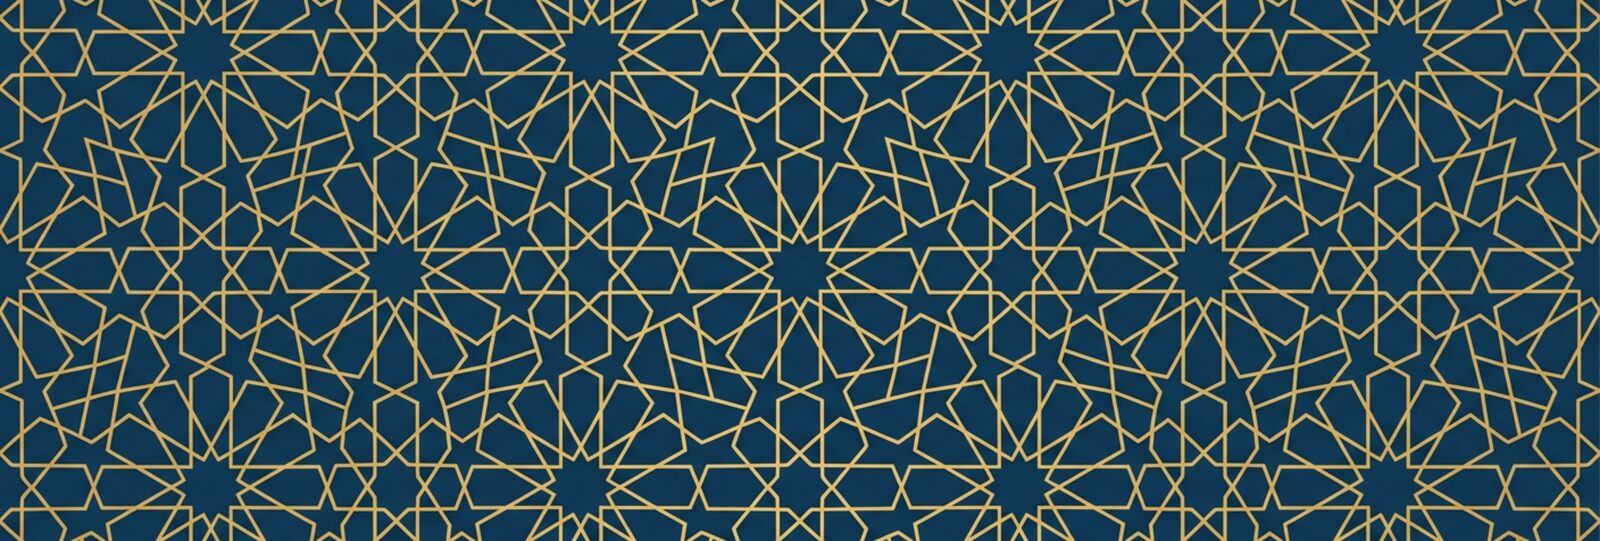
\includegraphics[width=21.4cm, angle=180]{assets/band-strip.jpg}};
  \end{scope}

  % عنوان
  \node[text=JAccentL, font=\JUIFont\bfseries\small]
    at ([yshift=-6.55cm]current page.north) {\JRTL{جزوهٔ جامعِ آموزشی}};
  \node[text=white, font=\VazirF\bfseries\fontsize{31}{42}\selectfont]
    at ([yshift=-7.95cm]current page.north) {\JRTL{عربی، زبانِ قرآن}};
  \node[text=JPrimaryL, font=\JUIFont\fontsize{12.5}{19}\selectfont]
    at ([yshift=-9.25cm]current page.north)
    {\JRTL{پایهٔ دوازدهم \\;{\color{JAccent}\textbullet}\; رشتهٔ علومِ انسانی}};

  % جداکنندهٔ طلایی
  \draw[JAccent, line width=0.9pt, opacity=0.85]
    ([yshift=-10.35cm]current page.north) ++(-2.9cm,0) -- ++(1.7cm,0);
  \draw[JAccent, line width=0.9pt, opacity=0.85]
    ([yshift=-10.35cm]current page.north) ++(2.9cm,0) -- ++(-1.7cm,0);
  \node[regular polygon, regular polygon sides=4, rotate=45,
    inner sep=1.6pt, fill=JAccent] at ([yshift=-10.35cm]current page.north) {};

  % مدالیونِ مرکزی
  \begin{scope}
    \clip ([yshift=-14.6cm]current page.north) circle (2.42cm);
    \node[inner sep=0pt] at ([yshift=-14.6cm]current page.north)
      {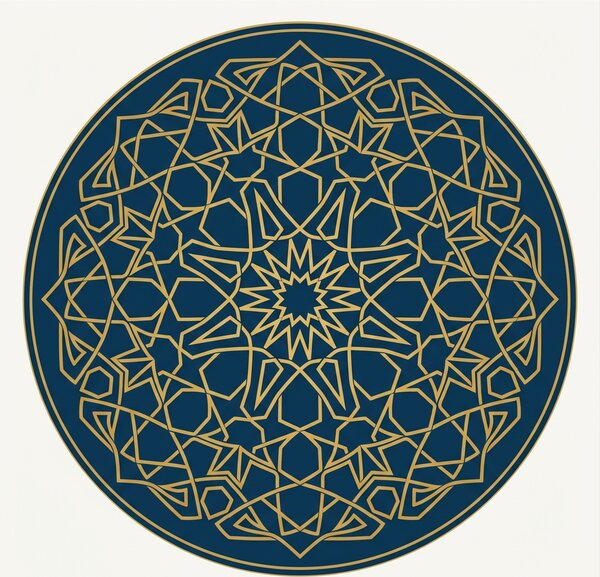
\includegraphics[width=5.1cm]{assets/medallion-trim.jpg}};
  \end{scope}
  \draw[JAccent, line width=1.1pt, opacity=0.9]
    ([yshift=-14.6cm]current page.north) circle (2.48cm);
  \draw[white, line width=0.5pt, opacity=0.25]
    ([yshift=-14.6cm]current page.north) circle (2.72cm);

  % اطلاعاتِ پایانیِ جلد: nodeهای مطلق، نه متنِ عادیِ صفحه
  \node[draw=JAccent, fill=JPrimary, rounded corners=5pt,
        line width=0.9pt, text=white, inner xsep=16pt, inner ysep=7pt,
        font=\JUIFont\bfseries\fontsize{12.5}{18}\selectfont]
    at ([yshift=-22.45cm]current page.north) {\JRTL{\JAuthor}};

  \node[draw=JAccent, fill=white, rounded corners=3pt,
        line width=0.7pt, text=JPrimary, inner xsep=7pt, inner ysep=3pt,
        font=\JUIFont\bfseries\footnotesize]
    at ([xshift=-5.0cm,yshift=-23.75cm]current page.north) {\JRTL{پنج درسِ کامل}};
  \node[draw=JAccent, fill=white, rounded corners=3pt,
        line width=0.7pt, text=JPrimary, inner xsep=7pt, inner ysep=3pt,
        font=\JUIFont\bfseries\footnotesize]
    at ([xshift=-1.65cm,yshift=-23.75cm]current page.north) {\JRTL{واژه‌نامهٔ جامع}};
  \node[draw=JAccent, fill=white, rounded corners=3pt,
        line width=0.7pt, text=JPrimary, inner xsep=7pt, inner ysep=3pt,
        font=\JUIFont\bfseries\footnotesize]
    at ([xshift=1.75cm,yshift=-23.75cm]current page.north) {\JRTL{درسنامهٔ قواعد}};
  \node[draw=JAccent, fill=white, rounded corners=3pt,
        line width=0.7pt, text=JPrimary, inner xsep=7pt, inner ysep=3pt,
        font=\JUIFont\bfseries\footnotesize]
    at ([xshift=5.05cm,yshift=-23.75cm]current page.north) {\JRTL{بانکِ تست و آزمون}};

  \node[text=JAccentL!88, font=\JUIFont\small, align=center,
        text width=16.5cm]
    at ([yshift=-24.75cm]current page.north) {\JRTL{\JBookNote}};
\end{tikzpicture}%
\newpage
